% High-frequency in-game dynamics from the recorded L2 (two nights, 50 game legs).
% Every number traces to data/research/pm_vol/hf_results.json, drift_sim.json or drift_tail.json
% (written by src/albert/research/pm_vol.py; report research-pm-vol-hf-20261109T221912Z).

The in-game sample has 50 game-winner legs (NBA 14, NCAAF 14, NFL 10, NHL 12), with 6{,}965
in-game minutes over two nights (\cref{sec:dyn-hf}). % source: hf_results.json:games
Every statistic is reported next to the matched M0 control of \cref{sec:dyn-control}, which has the
same games, windows, starting prices and spreads but no jumps and no stochastic volatility. Five
facts emerge.
\begin{enumerate}
\item The variance scales like Brownian motion from one second to five minutes, at a level set by
  the league.
\item The mid shows no measurable bid--ask bounce, unlike a quote re-rounded to the tick each
  second.
\item The shape is far from Gaussian at seconds and becomes nearly Gaussian only at about five
  minutes, because about half of the variance arrives in jumps.
\item Jump sizes follow Stern's fixed-score scaling in basketball but not in football or hockey.
\item There is no vol--price correlation beyond what M0 implies at minute scales.
\end{enumerate}

\subsubsection{Scale invariance and the variance signature}\label{sec:dyn-res-hf-scale}

\Cref{tab:dyn-hf-m0} reports the standardized innovation under the uniform clock at each horizon.
Variance is flat in the horizon. $\Var(\ustd)$ is 0.71, 0.77, 0.77, 0.73 and 0.77 at
  1, 5, 15, 60 and 300 seconds, so the Brownian time scaling holds across two and a half orders of
  magnitude. The level is below one ($t$ of $\ustd^2-1$ between $-3.5$ and $-5.1$, by game). With
  start spreads of at most 2\cents{} it is 0.66--0.77.

The level is set by the league, and the per-league values are also flat in the
  horizon. NBA games run above the uniform clock ($\Var(\ustd)$ of 1.17--1.33); NCAAF (0.47--0.54),
  NFL (0.57--0.64) and NHL (0.57--0.67) run below it. A plausible reading is that the scheduled end
  is a poor proxy for the remaining game clock: long stoppages in football and the buffer in the
  scheduled expiration both make $\tauexp$ too long.

The shape is not scale-invariant. Excess kurtosis falls from 151 at one second to 51,
  24 and 9 at 5, 15 and 60 seconds, and to 2 at five minutes; $P(|\ustd|>4)$ falls from 0.99\% to
  zero.
The control behaves differently. In the matched control the tick grid inflates
  $\Var(\ustd)$ to 2.64 at one second, falling to 1.02 at one minute, and kurtosis stays below 7.
% source: hf_results.json:m0, m0_sim

\begin{table}[t]
\centering
\begin{threeparttable}
\caption{In-game M0 test by horizon: data and matched tick-grid control}\label{tab:dyn-hf-m0}
\scriptsize
\setlength{\tabcolsep}{3pt}
% source: data/research/pm_vol/hf_results.json:m0, m0_sim (start_spread_max_c = 3 unless noted)
\begin{tabular}{rrcccccccc}
\toprule
 & & \multicolumn{5}{c}{Data} & \multicolumn{3}{c}{M0 control (1\cents{} grid)} \\
\cmidrule(lr){3-7}\cmidrule(lr){8-10}
$h$ (s) & Steps & $\Var(\ustd)$ & ($t$) & Exc.\ kurt. & $P(|\ustd|>4)$, \% & $\Var(\ustd)$, 2\cents & $\Var(\ustd)$ & Exc.\ kurt. & $P(|\ustd|>4)$, \% \\
\midrule
1 & 319{,}821 & 0.71 & ($-5.1$) & 151.3 & 0.99 & 0.66 & 2.64 & 6.3 & 2.97 \\
5 & 63{,}909 & 0.77 & ($-3.6$) & 51.1 & 0.99 & 0.74 & 1.42 & 1.1 & 0.47 \\
15 & 21{,}277 & 0.77 & ($-3.6$) & 23.7 & 0.79 & 0.76 & 1.16 & 0.2 & 0.06 \\
60 & 5{,}265 & 0.73 & ($-4.4$) & 9.0 & 0.53 & 0.73 & 1.02 & 0.1 & 0.00 \\
300 & 991 & 0.77 & ($-3.5$) & 2.0 & 0.00 & 0.77 & 1.07 & 0.0 & 0.00 \\
\midrule
\multicolumn{10}{l}{\emph{By league (data): $\Var(\ustd)$ at $h=$ 1, 5, 15, 60, 300\,s; excess kurtosis at 1, 60, 300\,s}} \\
\multicolumn{2}{l}{NBA (14 games)} & 1.17 & 1.33 & 1.31 & 1.26 & 1.29 & 62.6 & 3.2 & 0.2 \\
\multicolumn{2}{l}{NCAAF (14)} & 0.47 & 0.48 & 0.49 & 0.48 & 0.54 & 161.3 & 9.9 & 1.8 \\
\multicolumn{2}{l}{NFL (10)} & 0.57 & 0.61 & 0.64 & 0.62 & 0.59 & 167.4 & 7.6 & 2.6 \\
\multicolumn{2}{l}{NHL (12)} & 0.65 & 0.65 & 0.65 & 0.57 & 0.67 & 309.9 & 24.1 & 4.4 \\
\bottomrule
\end{tabular}
\begin{tablenotes}[flushleft]\footnotesize
\item Recorded Kalshi L2, nights of 7--8 and 8--9 November 2026; one game-winner leg per game, 50 games. Non-overlapping $h$-second steps under the uniform clock to the scheduled end; start spread $\le3$\cents{} (``2\cents'': $\le2$\cents), mid in $[0.03,0.97]$; end spread $\le10$\cents.
\item ($t$): $t$-statistic of $\E[\ustd^2-1]$, clustered by game. The control simulates an M0 path per game and quotes it on the 1\cents{} grid with that game's spreads (\cref{sec:dyn-control}).
\item In the league rows, the columns under Data hold $\Var(\ustd)$ at the five horizons and the control columns hold the data's excess kurtosis at 1, 60 and 300\,s.
\end{tablenotes}
\end{threeparttable}
\end{table}

\Cref{fig:dyn-signature} shows the variance signature.
Realized variance of the mid per in-game hour is flat, between 453 and
  524\,c$^2$ for sampling intervals from 1 to 600 seconds. Fitting \cref{eq:dyn-signature} gives
  $\sigma^2=503$\,c$^2$ per hour and a noise variance at its lower bound of zero.
The control has the textbook signature: 1{,}148\,c$^2$ at one second,
  falling to 608 at one minute, with $\eta=0.27$\cents{} and noise accounting for 46\% of
  one-second realized variance.
% source: hf_results.json:signature, signature_fit, signature_sim, signature_fit_sim
Kalshi in-game mids therefore do not flicker across the tick. The book moves when the price moves,
and quote discreteness appears as stickiness rather than bounce. The slight rise of realized
variance from 1 to 10 seconds (453 to 524\,c$^2$) is mild positive autocorrelation at the seconds
scale: quotes take a few seconds to adjust. Beyond about ten seconds increments are uncorrelated.
For realized-variance estimation this means sparse sampling corrections
\citep{zhang2005,aitsahalia2005,hansenlunde2006} are unnecessary on this venue at these horizons.

\begin{figure}[t]
\centering
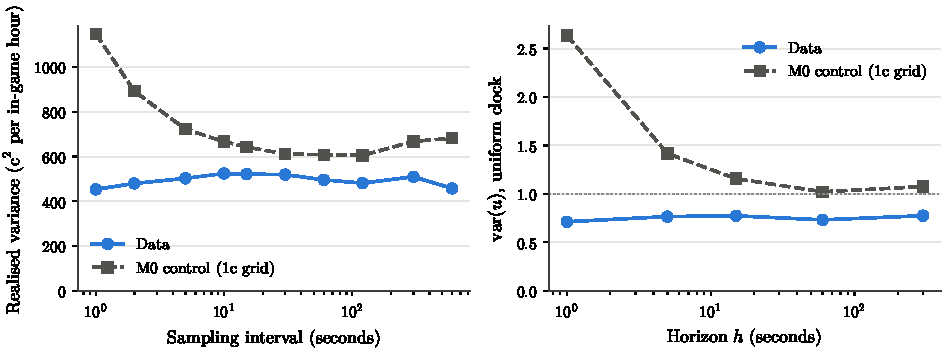
\includegraphics[width=\textwidth]{figures/fig_dyn_signature.pdf}
\caption{In-game variance signature and time scaling, recorded L2, two nights, 50 games. Left: realized variance of the mid per in-game hour against the sampling interval. Right: $\Var(\ustd)$ under the uniform clock against the horizon; the dotted line marks one. Dashed: the matched M0 control, quoted on the 1\cents{} grid with each game's own spreads.}
\label{fig:dyn-signature}
\end{figure}

\subsubsection{The probit-drift shortfall}\label{sec:dyn-res-drift}

In the hourly data the outward probit drift, which keeps $\pr$ a martingale under M0, is only a
fraction of its predicted size. The instrumental-variable estimates of \cref{sec:dyn-clock} are no
closer to one, so quote noise in $\Zt_t$ does not explain it. \Cref{tab:dyn-drift} and
\cref{fig:dyn-drift} test whether the price grid does.
In weather, Mentions, Elections and Science \& Technology,
  M0 paths quoted on the 1\cents{} grid with the real spreads reproduce the measured slope (data
  0.57, 0.42, 0.35, 0.47; tick control 0.32, 0.48, 0.37, 0.53). There the shortfall comes from the
  grid, the 0.5\cents{} probit clip and, for weather, the steep clock, which together truncate
  outward moves near the edges.
Ticks explain it only in part for Entertainment (0.35 against
  0.71) and Politics (0.73 against 1.03).

They do not explain it for sports: pre-game hourly
  0.11 ($\text{s.e.}=0.08$) against 0.93, and in-game L2 0.46 (0.21) at 60 seconds and 0.40 (0.25)
  at 300 seconds, against 1.37 and 0.87.
Stale quotes add nothing. Re-quoting only in hours with real activity gives the same
  slopes as the tick control.
% source: drift_sim.json (p_range = all); hf_results.json:drift_hf

Three further results locate the residual shortfall and rule out under-reaction as its source.
The price itself does not drift. The mean of $\sgn(\Zt_t)\Delta\pr$ is
  $+0.003$\cents{} per hour pre-game ($t=1.3$) and $-0.004$\cents{} per minute in-game ($t=-0.1$).
  A Gaussian M0 price with the measured Z-drift would drift by $-0.020$\cents{} per hour pre-game,
  which lies outside the confidence band of the measured value.
The shortfall is not in the tails. Trimming with windows that bias in opposite
  directions leaves the slope low: pre-game 0.13 and 0.05, in-game 0.68 and 0.61 at 60 seconds.
The core carries little of the clock. Within the core ($|\ustd|\le2$),
  $\E(\Delta\Zt)^2$ is only 8\% (pre-game), 19\% (Mentions, Entertainment) and 34\% (in-game, 60\,s)
  of the clock increment $L$. Within that core, the local second-order martingale ratio
  $\E[\sgn(\Zt)\Delta\Zt]/\E[\tfrac12|\Zt|(\Delta\Zt)^2]$ is 1.35--2.26.
% source: drift_tail.json

So the diffusive part of the motion drifts outward at least as much as a martingale requires given
its own variance. The shortfall arises because most of the clock's information arrives in jumps,
and the Gaussian compensator $e^{L/2}$ of M0 overstates the drift needed when the variance is
jump-borne. That is the M2 regime of \cref{sec:model}, not under-reaction. The only under-reaction
we find is the seconds-scale adjustment visible in the signature plot.

\begin{table}[t]
\centering
\begin{threeparttable}
\caption{Probit-drift slope: data, tick-grid controls and where the shortfall lies}\label{tab:dyn-drift}
\scriptsize
\setlength{\tabcolsep}{2.5pt}
% source: data/research/pm_vol/drift_sim.json (p_range = all), hf_results.json:drift_hf, drift_tail.json
\begin{tabular}{lcccccccc}
\toprule
 & \multicolumn{4}{c}{Slope (M0 $=1$)} & Trimmed slope & Core & Local & $\E[\sgn(\Zt)\Delta\pr]$ \\
\cmidrule(lr){2-5}
Sample & Data (s.e.) & Tick (s.e.) & Stale & True & $|\ustd|\le2$ / $|\Delta\Zt|\le2$sd & $\E(\Delta\Zt)^2/\E L$ & ratio & \cents{} ($t$) \\
\midrule
Weather (1\,h) & 0.57 (0.05) & 0.32 (0.01) & 0.28 & 0.57 & 0.69 / 0.62 & 0.49 & 1.35 & $-0.021$ ($-1.0$) \\
Mentions (1\,h) & 0.42 (0.12) & 0.48 (0.10) & 0.43 & 0.88 & 0.39 / 0.37 & 0.19 & 1.86 & 0.026 (1.5) \\
Elections (1\,h) & 0.35 (0.10) & 0.37 (0.12) & 0.34 & 0.84 & -- & -- & -- & 0.006 (1.6) \\
Sci.\ \& Tech.\ (1\,h) & 0.47 (0.16) & 0.53 (0.10) & 0.41 & 0.69 & -- & -- & -- & 0.026 (1.8) \\
Entertainment (1\,h) & 0.35 (0.15) & 0.71 (0.10) & 0.71 & 1.16 & 0.25 / 0.25 & 0.19 & 1.82 & $-0.003$ ($-0.9$) \\
Politics (1\,h) & 0.73 (0.11) & 1.03 (0.21) & 0.99 & 1.11 & 0.58 / 0.56 & 0.22 & 2.19 & $-0.010$ ($-0.9$) \\
Sports pre-game (1\,h) & 0.11 (0.08) & 0.93 (0.09) & 0.92 & 1.06 & 0.13 / 0.05 & 0.08 & 1.43 & 0.003 (1.3) \\
In-game L2 (60\,s) & 0.46 (0.21) & 1.37 (0.39) & -- & 1.29 & 0.68 / 0.61 & 0.34 & 2.26 & $-0.004$ ($-0.1$) \\
In-game L2 (300\,s) & 0.40 (0.25) & 0.87 (0.32) & -- & 0.93 & 0.51 / 0.47 & 0.48 & 1.35 & 0.031 (0.1) \\
\bottomrule
\end{tabular}
\begin{tablenotes}[flushleft]\footnotesize
\item Slope of $\tilde\Zt_{t+h}-\tilde\Zt_t$ on $\tilde\Zt_t(e^{L/2}-1)$, steps with $L\le2$. Hourly rows: estimation sample (before 1 October 2026), category clock fitted on the estimation sample. L2 rows: in-game, uniform clock. Standard errors clustered by event (hourly) or game (L2).
\item \emph{Tick}, \emph{Stale}, \emph{True}: M0 paths simulated on the same grids, quoted on the 1\cents{} grid with the real spreads, re-quoted only in hours with real activity, or not quoted (\cref{sec:dyn-control}).
\item \emph{Trimmed}: windows centred on M0's mean (biases toward 1) and on zero drift (biases toward 0). \emph{Core} and \emph{Local ratio}: within $|\ustd|\le2$; local ratio $=\E[\sgn(\Zt)\Delta\Zt]/\E[\frac12|\Zt|(\Delta\Zt)^2]$ on $|\Zt|\ge0.5$ (one for a martingale). The trimming diagnostics were run for the categories shown.
\item Last column: per hour (hourly rows) or per step (L2 rows), $t$ clustered as above.
\end{tablenotes}
\end{threeparttable}
\end{table}

\begin{figure}[t]
\centering
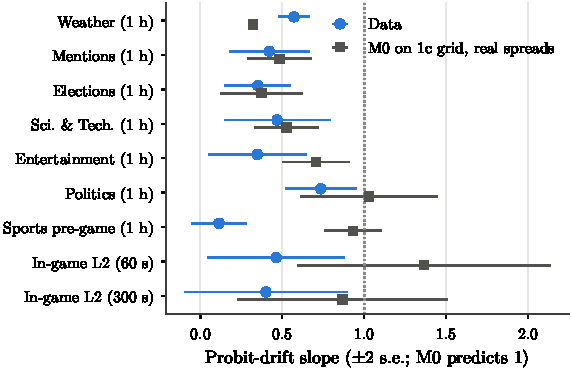
\includegraphics[width=0.66\textwidth]{figures/fig_dyn_drift.pdf}
\caption{Probit-drift slope ($\pm2$ standard errors, clustered by event or game) in the data and in M0 paths quoted on the 1\cents{} grid with the real spreads. Hourly rows: estimation sample (before 1 October 2026). L2 rows: in-game, two nights. The dotted line is M0's prediction. Ticks reproduce the shortfall in weather, Mentions, Elections and Science \& Technology but not in sports.}
\label{fig:dyn-drift}
\end{figure}

\subsubsection{Jumps and Stern's scaling}\label{sec:dyn-res-hf-jumps}

Panel A of \cref{tab:dyn-hf-jumps} measures how much of the in-game variance arrives in jumps.
Bipower variation misses 59\%, 53\% and 48\% of realized variance at 5, 10 and
  15 seconds; the median game shows 61--66\%. In the control, bipower variation misses only 8--16\%:
  the familiar small-sample and discreteness bias of bipower tests on a tick grid. The excess over
  the control, about 40--45 percentage points, is a conservative estimate of the in-game jump share.
Threshold jumps (more than four local standard deviations and at least 2\cents) carry
  51--68\% of realized variance, against 1\% or less in the control.
At 10 seconds we detect 859 jumps in 50 games, about 7.4 per
  in-game hour, with a median size of 3.5\cents. The control produces 58.
These shares are consistent with the hourly EM estimate for in-game sports (0.65--0.66 of
$\sum(\Delta\pr)^2$, \cref{tab:dyn-sv}).
% source: hf_results.json:jumps, jumps_sim, n_jumps_sim_10s, stern

For a fixed score increment, Stern's Brownian game model implies that the price jump scales as
$\varphi(\Zt)/\sqrt{\tauexp}$ (Panel B).
In the NBA the log--log slope is $1.08$ ($\text{s.e.}=0.09$), as predicted.

For the NFL, NCAAF and NHL the slope is 0.50 (0.10), 0.56 (0.08) and 0.65 (0.16); the
  pooled slope with league fixed effects is 0.69 (0.07).

Basketball scoring is frequent and small, close to the Brownian limit. Touchdowns, field goals and
goals are large and discrete, and their price impact depends on the game state through more than
$\varphi(\Zt)$. Measuring $\tauexp$ to the scheduled end rather than the game clock also flattens the
slope.

\subsubsection{Leverage at minute scales}\label{sec:dyn-res-hf-lev}

At horizons of one, two and five minutes (Panel C), the vol--price correlation in probit units is
$+0.016$, $+0.003$ and $+0.045$, all with $|t|<1.4$, matching the control's zero. In price units
the correlation is negative ($-0.056$ to $-0.088$). M0 itself produces this mechanically, because
$\varphi(\Zt)$ rises as the price moves toward $1/2$; the control gives $-0.07$ to $-0.17$. The
hourly in-game correlation of $-0.11$ in probit units (\cref{tab:dyn-sv}) therefore has no
counterpart at minute scales. If it is structural, it reflects game-state changes over hours, such
as the late stages of close games, rather than short-run feedback.
% source: hf_results.json:leverage, leverage_sim

\begin{table}[t]
\centering
\begin{threeparttable}
\caption{In-game jumps, Stern scaling and leverage}\label{tab:dyn-hf-jumps}
\footnotesize
\setlength{\tabcolsep}{3.5pt}
% source: data/research/pm_vol/hf_results.json:jumps, jumps_sim, stern, leverage, leverage_sim
\begin{tabular}{lccccc}
\toprule
\multicolumn{6}{l}{\emph{A. Share of realized variance from jumps}} \\
$h$ (s) & Bipower & Bipower, med.\ game & Bipower, control & Threshold & Threshold, control \\
\midrule
5 & 0.59 & 0.66 & 0.16 & 0.68 & 0.005 \\
10 & 0.53 & 0.61 & 0.09 & 0.57 & 0.009 \\
15 & 0.48 & 0.63 & 0.08 & 0.51 & 0.010 \\
\midrule
\multicolumn{6}{l}{\emph{B. Jump size against $\varphi(\Zt)/\sqrt{\tauexp}$, 10\,s jumps (Stern: slope 1)}} \\
League & Jumps & Games & Med.\ $|\Delta\pr|$ (\cents) & Price slope (s.e.) & Probit slope (s.e.) \\
\midrule
Pooled (league f.e.) & 859 & 50 & 3.5 & 0.69 (0.07) & 0.72 (0.10) \\
NBA & 236 & 14 & 4.0 & 1.08 (0.09) & 1.92 (0.12) \\
NCAAF & 187 & 14 & 3.5 & 0.56 (0.08) & 0.41 (0.14) \\
NFL & 284 & 10 & 3.5 & 0.50 (0.10) & 0.55 (0.11) \\
NHL & 152 & 12 & 3.0 & 0.65 (0.16) & 0.59 (0.21) \\
\midrule
\multicolumn{6}{l}{\emph{C. Leverage, \cref{eq:dyn-lev} with $x$ for $\ustd$ ($t$)}} \\
$h$ (s) & Steps & $x=\ustd$, data & $x=\ustd$, control & $x=\Delta\pr$, data & $x=\Delta\pr$, control \\
\midrule
60 & 4{,}447 & 0.016 (0.9) & 0.000 (0.0) & $-0.056$ ($-2.3$) & $-0.068$ ($-2.9$) \\
120 & 2{,}181 & 0.003 (0.1) & $-0.007$ ($-0.3$) & $-0.088$ ($-2.8$) & $-0.106$ ($-3.5$) \\
300 & 822 & 0.045 (1.4) & 0.008 (0.2) & $-0.075$ ($-1.7$) & $-0.165$ ($-4.7$) \\
\bottomrule
\end{tabular}
\begin{tablenotes}[flushleft]\footnotesize
\item Recorded L2, two nights, 50 games; steps with start spread $\le3$\cents{} and mid in $[0.03,0.97]$ (Panel C: $[0.1,0.9]$). Control: M0 paths quoted on the 1\cents{} grid with each game's spreads.
\item A: bipower share $=(RV-BV)/RV$; threshold jumps have $|\ustd|>4$ local bipower standard deviations and $|\Delta\pr|\ge2$\cents. B: price slope of $\log|\Delta\pr|$ on $\log[\varphi(\Zt)/\sqrt{\tauexp}]$; probit slope of $\log|\Delta\Zt|$ on $\log\tauexp^{-1/2}$; OLS, standard errors clustered by game. C: correlation of $\sgn(\Zt_t)x_t$ with the mean $|x|$ over the next five steps; $t$ clustered by game; negative values mean volatility rises after moves toward $1/2$.
\end{tablenotes}
\end{threeparttable}
\end{table}

\paragraph{Limitations.}
\begin{itemize}
\item The sample covers two nights and 50 games, so league-level estimates rest on 10--14 games
  each.
\item The in-game window comes from the schedule and can include a few pre-kickoff minutes, which
  pushes $\Var(\ustd)$ down.
\item $\tauexp$ is measured to the scheduled settlement time, not the game clock.
\item Without a score feed, ``jumps'' are price discontinuities, not verified scoring events.
\end{itemize}
